\chapter{Преглед на предметната област} % Main chapter title

\label{Chapter2} 

%----------------------------------------------------------------------------------------

\section{Въведение}

През 1959 г. Артър Самюел определя машинното самообучение като „Поле на проучване, което дава на компютрите възможността да учат, без да бъдат експлицитно програмирани“. То изследва проучването и изграждането на алгоритми, които да правят прогнози чрез данни и от които да може да се учи. Машинното самообучение използва събрани исторически данни  за изграждането на модел, който в последствие да може да се използва върху нови данни.

Машинното самообучение се използва в широка гама от изчислителни задачи, където програмирането на експлицитни алгоритми е неосъществимо. Примерните приложения включват филтриране на спам, оптично разпознаване на символи, търсачки и компютърно зрение.

В областта на аналитични данни, машинното самообучение се използва за разработване на сложни модели и алгоритми, които се поддават на прогнозиране. Тези аналитични модели позволяват изследователи, учени и инженери да получават надеждни, повтаряеми решения и резултати.

\section{Разпознаване на изображения: мотивация и история}

През 1963 година в докторската си теза Л. Робъртс \cite{Solids1963} разглежда в детайли как машините могат да възприемат дадени триизмерни обекти от изображение. Той анализира очертанията на обектите и различните перспективи на заснемане. През 1987 година учени от Кеймбридж (Масачузетс) описват разпознаване на обекти с използване на изкуствен интелект \cite{Alignment1987}. Намират се изключително много приложения на разпознаването на обекти в изображения и все повече и повече данни започват да бъдат налични.

В края на 70-те и началото на 80-те невронните мрежи започват да добиват все по-голяма популярност и започват да се прилагат в множество области. Конволюционните невронни мрежи са вдъхновени от зрението на животните в природата. В началото на 21 век се случват няколко много важни неща, които предразполагат развитието на пазара в сферата на автоматичното класифициране на изображения.

Едно от тях е, че се намират начини за използване на видео картата за изчисления в невронните мрежи, което значително подобрява времето на изпълнение. Със създаването и популяризирането на социалните мрежи броят на картинките е огромен: всеки ден над 350 милиона снимки се качват само във Facebook \cite{FacebookFacts}.

Активното използване на автоматично разчитане на изображения се прилага активно в днешни дни. То служи за разпознаване на номера от автомобили, пощенски кодове и чекове. Все с по-голяма сила навлиза разпознаването на пръстови отпечатъци за идентификация \cite{Fingerprints}.

Със особено влияние са алгоритмите за локализиране и разпознаване на лице на хора. При наличието на много улични камери такъв алгоритъм разполага с възможност да търси в гигантско количество информация.

С увеличаването на интернет потребителите се увеличават и заплахите в електронния свят. Публично се разпространяват изображения, свързани с насилие, детска порнография и други нецензурирани материали. Автоматичното разпознаване на изображения идва на помощ при засичането на подобни нередности.


%----------------------------------------------------------------------------------------

\section{Невронни мрежи}

Невронната мрежа е модел за обработка на информация, вдъхновен от изучаването на биоелектричните мрежи в мозъка на човека и животните, образувани от неврони и техните синапси. В наши дни учените често наричат изкуствените невронни мрежи просто невронни мрежи.

Математическият аналог на биологичната невронна мрежа представлява множество от взаимносвързани прости изчислителни елементи (неврони). Всеки неврон приема сигнали от другите (под формата на числа), сумира ги, като сумата минава през активационна функция, и така определя своята активация (степен на възбуда), която се предава по изходящите връзки към другите неврони. Всяка връзка има тегло, което, умножавайки се със сигнала, определя неговата значимост (сила). Теглата на връзките са аналогични на силата на синаптичните импулси, предавани между биологичните неврони. Отрицателна стойност на теглото съответства на потискащ импулс, а положителна – на възбуждащ. \ref{fig:NeuralNetwork} илюстрира примерна невронна мрежа.

\begin{figure}[H]
\centering
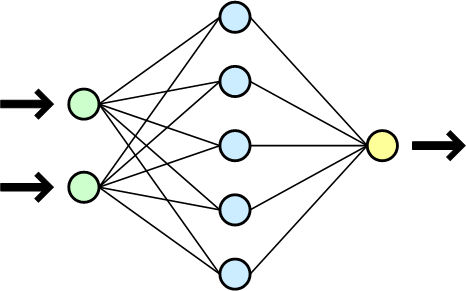
\includegraphics[width=250px]{Figures/Neuralnetwork.png}
\caption{Невронна мрежа}
\label{fig:NeuralNetwork}
\end{figure}

В невронната мрежа обикновено винаги съществуват входен и изходен слой от неврони, във входния се въвежда информацията към мрежата, след това сигналите от входните неврони преминават през един или няколко слоя от междинни (скрити) неврони, според топологията на невронната мрежа, като сигналите накрая стигат до изходния слой, откъдето се чете получената информация.

Теглата на връзките между невроните определят функционалността и поведението на невронната мрежа. За да бъде една невронна мрежа използваема и приложима към даден проблем, тя трябва да бъде предварително обучена.

Обучаването на една невронна мрежа се осъществавя с използване на тренировъчни данни, като в процеса на обучение се променят теглата на връзките между невроните търсейки се най-оптимални тегла спрямо тренировъчните данни. Най-разпространеното правило за това е метода на обратното разпространение на сигнал за грешка (back-propagation), където за всеки изходен неврон се изчислява разликата от желаното му поведение, като се формира сигнал за грешка, който се движи назад към входния слой и по пътя си променя теглата на връзките така, че при следващата активация на мрежата грешката да бъде по-малка от сегашната.

Невронните мрежи много се доближават до нашите мозъци по начина си на функциониране.  Изчисленията не се извършват на едно централно място, а са разпределени по цялата мрежа. Това прави мрежата изключително гъвкава, като тя продължава да работи дори когато от нея умишлено са премахнати изчислителни елементи. За сравнение, фон Ноймановата архитектура престава да функционира ако от нея липсва дори един елемент.

За съжаление, дори този модел на човешкия ум не е перфектен. Повечето съществуващи към момента изкуствени невронни мрежи не могат да моделират ефекта на хормоните върху мозъка. Освен това се оказва, че за да можем математически да опишем една изкуствена мрежа, в нея трябва да се спазват определени правила, например сигналите да се движат от входния към изходния слой, но не и обратно. (Съществуват и изкуствени мрежи, които са циклични, но поради повишената им сложност все още не са добре изучени.) Може би най-големият недостатък на невронните мрежи е, че тяхното обучение изисква множество повторения, а в много случаи човек научава дадена информация след като е бил изложен на нея само веднъж.

%----------------------------------------------------------------------------------------

\section{Задълбочено обучение (deep learning)}

Задълбоченото обучение е направление в машинното самообучение, който се основава на алгоритми, които целят да изградят абстракция от високо ниво на данните. Ако разгледаме един много прост случай може да имаме две множества неврони: едни, които получават входен сигнал и втори, които изпращат изходящ сигнал. Когато първият слой получи вход, той предава модифицирана версия на входа към следващия слой. При по-дълбока мрежа, има много слоя между входния и изходния, което позволява на алгоритъма за използва множество обработващи слоя, състоящи се от много трансформации. \cite{DeepLearningMethods} \cite{DeepArchitectures}

Дълбокото учение е част от по-голяма група методи в машинното самообучение, които се основават на обучение върху изгледа на данни. Наблюдение (например картинка) може да се представи по много начини като например вектор от интензивността на пикселите или по по-абстрактен начин като множество от ъгли, региони с определена форма и още много други. Някои изгледи са по-добри от други по отношение на опростяване на обучението. Една от основните дейности на задълбоченото обучение е, че се премахва нуждата от ръчно изваждане на модели от хора. На тяхно място се използват ефективни алгоритми за обучение и йерархично автоматично изграждане на модели.

Разработките в тази насока се стремят да се намерят тези модели в огромен обем необработени данни. Някои модели са вдъхновени от напредъка в неврологията и се основават на интерпретации на обработката на информация и начините на комуникация в нервната система.

Различни видове архитектури като Невронни мрежи, Конволюционни невронни мрежи, Deep belief мрежи и рекурентни невронни мрежи са прилагани в области като разпознаване на реч, обработка на естесвен език, разпознаване на звуци, биоинформатика, където те достигат най-точни резултати от всички използвани методи.

%----------------------------------------------------------------------------------------

\section{Конволюционни Невронни мрежи}

Този вид невронни мрежи за вдъхновени от визуалния кортекс при животните. Отделни неврони отговарят за стимулирането на ограничен район на действие, който се нарича област на възприемане. Когато полето на възприемане на даден неврон бъде задействано, неговият отговор може да бъде изчислен математически чрез конволюционна операция (convolutional). Вдъхновени са от биологични процеси и са вариация на многопластов перцептрон, който използва минимално количество предварителна обработка. Те са най-приложими в обработката на изображения и видеа, препоръчващите системи и обработката на естествен език. \cite{CNN_2} \cite{CNN_3}


\subsection{Област (поле) на възприемане}
През 50-те и 60-те години на 20 век труд на Хубел и Визел показва, че визуалния кортекс на котките и маймуните съдържа неврони, които индивидуално реагират на малки региони от визуалното поле. Регионът от визуалното поле, в който съдържанието въздейства на специфични неврони се нарича област (поле) на възприемане. Съседните клетки имат подобни и припокриващи се полета на възприемане. Размерът и мястото на областта на възприемане варира из корпуса, за да формира пълна карта на визуалното пространство. \cite{CNN_1}

\subsection{Специфични особености}
Въпреки, че стандартните невронни мрежи могат успешно да бъдат приложени за разпознаване на изображения, те имат сериозен недостатък при уголемяване на размерите на изображенията. Например при изображение с размери 32x32 пиксела и 3 цветови канала един пълно свързан неврон би имал 32*32*3=3072 тегла. При изображение с размери 500x500 броят им би бил 750 000. При наличието на следващ слой със същата големина броят на връзките би бил 562 500 000 000.
Освен това тази архитектура третира пиксели, които са раздалечени по един и същи начин като пиксели, които са един до друг. Очевидно пълната свързаност на невроните не е добро решение при задачата за разпознаване на изображения. Като следствие огромният брой параметри води до прекомерно нагаждане (overfitting). 
Конволюционните невронни мрежи имат следните специфични осоености
\begin{enumerate}
\item \textbf{3 измерения на невроните}. Слоевете имат неврони, организирани в 3 измерения: ширина, височина и дълбочина. Невроните във всеки слой са свързани само с малък брой от невроните в предишния слой (област на възприемане). Различни видове слоеве (както локално така и напълно свързани) се обединяват за да организират конволюционна невронна мрежа.
\item \textbf{Локална свързаност}: следвайки концепцията на полето на възприемане, този вид невронни мрежи използват локална свързаност като принуждават невроните от последователните слоеве да комуникират само с близките до тях съседи. По този начин архитектурата осигурява това, че научените "филтри" продуцират най-силна връзка при взаимодействие между близки неврони. Нареждането на много подобни връзки води до нелинейни филтри, които стават все по-глобални. Това позволява на мрежата първо да намери отличителни черти на малка част от входа и след това да види как те са приложени в по-голямо изображение.
\item \textbf{Споделени тегла}: Всеки филтър се прилага върху цялото визуално поле. Където се използват, тези единици споделят едни и същи тегла. Това означава, че всички неврони в даден слой засичат точно един и същи модел на свързаност. По този начин се позволява моделът да бъде намерен независимо къде се намира върху визуалното поле.
\end{enumerate}
Заедно тези свойства позволяват на конволюционните невронни мрежи да постигнат по-добра генерализация при визуалните проблеми. Споделянето на теглата драстично намалява броя на параметрите, които трябва да се обучат. По този начин се намаляват хардуерните изисквания за използване на невронната мрежа. Това от своя страна позволява тренирането на по-големи и по-мощни мрежи. 

\subsection{Видове слоеве}
Конволюционните невронни мрежи използват някои различни слоеве в сравнение със стандартните невронни мрежи. Такива са конволюционният слой, обединяващият слой и слоят на ректифицираните линейни единици (ReLU).

\ref{fig:ConvNeuralNetwork} показва примерна архитектура на конволюционна невронна мрежа.

\begin{figure}[H]
\centering
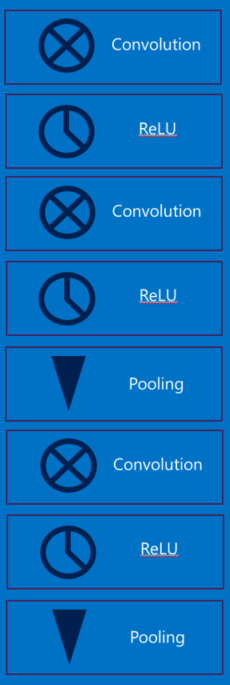
\includegraphics{Figures/cnn12.png}
\caption{Архитектура на конволюционна невронна мрежа \cite{CNN_blog}}
\label{fig:ConvNeuralNetwork}
\end{figure}

\subsubsection{Конволюционен слой}
Това е основата на този тип невронни мрежи. Параметрите на този слой са множество от самообучаващи се филтри, които имат малко поле на възприемане, но се разширяват до пълната дълбочина на входните параметри. При всяко предаване едно ниво напред всеки филтър създава своя карта в зависимост от това дали се среща или не по цялата ширина и височина на входа. Това означава, че се търси къде този филтър е наличен в подадения вход и се връща като резултат двуизмерна активационна карта, указваща местата на филтъра. Като резултат мрежата научава филтри, които се активират при специфичен модел на някоя позиция от входа.
Като се обединят активационните карти на всички филтри по измерението за дълбочина се оформя пълният изход от конволюционния слой. Всяка единица от изхода може да се интерпретира като резултат от неврон, който отговаря за малък регион от визуалното поле и споделя параметри с неврони от същата активационна карта.

Когато входните данни са от много високо измерение (както изображенията) не е практично да се свързват неврони с всички неврони от предходния слой, защото такава архитектура не взима предвид близостта на данните (например дали 2 пиксела са един до друг или раздалечени). Всеки неврон е свързан само с малък регион от входните данни. Големината на тези региони е хиперпараметър, който се нарича област на възприемане на неврона. Връзките са локални по отношение на ширина и височина, но винаги са по цялата дълбочина на входните данни. Такава архитектура гарантира, че научените филтри имат най-силно въздействие върху резултата.  

Три хиперпараметъра контролират размера на изхода на конволюционния слой: дълбочина, стъпка на алокиране и брой колони с добавени нули.
Дълбочината на изхода контролира броя неврони в слоя, които са свързани със същия регион от входния слой. Всички тези неврони ще се научат да се активират за различни модели на входа. Например, ако първият конволюционен слой приема необработено изображение като вход, различните неврони разположени в дълбочина може да се активират при наличие на различни ъгли, цветове или други форми. Стъпката (stride) се грижи за това как се оформят колоните в дълбочина около измеренията ширина и височина. Когато съпката е 1 се образува нова колона неврони, които са свързани само до единиците на разстояние 1. Това води до пренатоварване на полетата на възприемане между колоните и също така до огромни размери на изхода. Понякога е удобно да изместим входните данни като добавим нули на граничните стойности. Колко колони с нули ще добавим е третият хиперпараметър. Той ни дава контрол да определеми размера на изхода. 

В конволюционните слоеве се използва схема на споделяне на параметри  за контрол на броя на свободните параметри. То се основава на следното: ако даден модел е полезен в определен регион, то той би бил полезен дори да е намерен и на друга позиция. Тъй като всички неврони в един изрязък по отношение на дълбочина споделят един и същи параметри, изходът от всяка част от конволюционния слой може да се изчисли като конволюция от теглата на невроните към входните данни. Следователно, често срещано е да наричаме множество от тегла филтър (или ядро), който е свързан с вхдоните данни. Резултатът от конволюцията е активационна карта, и множеството такива карти за всеки филтър се напасват заедно по отношение на дълбочината за да генерират изходните данни. 
Важно е да се отбележи, че понякога споделянето на параметри може да не е подходящо. Такъв пример е когато входните изображения за невронната мрежа имат нещо специфично в центъра на изображенията и ние очакваме филтрите да бъдат намерени точно в централната част. Пример на практика е разпознаване на лица, където лицата са в центъра на изображението. В този случай избягваме споделянето на параметри и просто разчитаме на локално свързани слоеве.

\subsubsection{Обединяващ (Pooling) слой}
Друга важна концепция в конволюционните невронни мрежи е обединяването (pooling), което е вид нелинейно намаляване на пространство. Има няколко нелинейни функции, които имплементират обединяването. Най-популярната от тях е max pooling \ref{fig:MaxPooling}. При нея изображението се разделя на множество от непресичащи се правоъгълници и за всеки такъв регион връща максимума. Интиутивното обяснение е, че щом даден модел е бил намерен, неговото точно местоположение не е от толкова голямо значение колкото относителното му местоположение спрямо други модели. Основната роля на този слой е прогресивно да намали размера на данните в мрежата и следователно да се избегне прекомерното нагаждане. 
Този слой се изпълнява независимо за всяка дълбочина на входа и променя размерите независимо. Най-често срещаната форма в прилагане на pooling функция с филтри с размери 2x2 като по този начин се изоставят 75\% от активациите. По този начин всяка операция за максимизиране ще търси най-голямото от 4 числа. Измерението за дълбочина остава непроменено.
Други видове функции, които биха могли да бъдат приложени са средно аритметично намаляване и L2-нормализация. До скоро средно аритметичното намаляване е било предпочитано, но в последните години максимизирането дава по-добри резултати в практиката.

\begin{figure}[H]
\centering
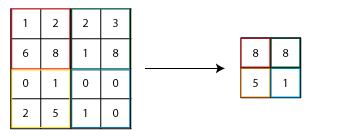
\includegraphics{Figures/Max_pooling.png}
\caption{Обединяващ (pooling) слой}
\label{fig:MaxPooling}
\end{figure}

\subsubsection{Слой на ректифицираните линейни единици (ReLU - Rectified Linear Units)}
Това е слой от неврони, който прилага активационната функция f(x)=max(0,x). Той повишава нелинейните свойства на функцията за взимане на решения и като цяло на мрежата без да оказва влияние на областите на възприемане на конволюционния слой.
Използват се и други функции за повишаване на нелинейността. Например f(x)=tanh(x) и f(x)=|tanh(x)|. ReLU е най-предпочитана в сравнение с другите функции, защото прави процеса на обучение на мрежата много по-кратък и няма големи разлики по отношение на точността.

\subsubsection{Напълно свързан слой}
Накрая след няколко конволюционни и обединяващи слоя взимането на решения се осъществява от напълно свързаните слоеве. Невроните в тях имат връзки със всички активации в предишния слой както при стандартните невронни мрежи. Тяхната активация би могла да се пресметне чрез матрица на умноженията, последвана от контролирано отклонение.

\subsubsection{Слой на наказанията}
Този слой указва как мрежата наказва разликата между предсказаните и истинските стойности и обикновено е последният слой в мрежата. Има различни функции за наказание в зависимост от конкретната задача. Softmax е една от тях и се използва, когато трябва да се предскаже 1 от няколко взаимно изключващи се класа. Това е и конкретният случай. Крос ентропичен сигмоид се използва при предсказване на K независими вероятности в диапазона [0,1].

\subsection{Избор на хиперпараметри}
\subsubsection{Брой филтри}
Тъй като с навлизане в невронната мрежа размерът на данните се намалява е удачно да имаме по-малко филтри в началото и повече в края. За да се уеднакви изчислителното време във всеки слой произведението на броя пиксели и броя модели е почти константно из всичките слоеве. За да се запази входната информация трябва да се осигури, че броят активации не трябва да намалява от един слой към следващия.

\subsubsection{Форма на филтрите}
Има много различни форми на филтрите и обикновено се избират в зависимост от входните данни.

\subsubsection{Максимални размери на формата за обединяване}
Обикновено обединяването се извършва върху 2x2 пиксела. При огромни входни данни може да бъде 4x4. Това обаче може да доведе до премахването на твърде много важна информация.

\subsection{Методи за регуларизация}

В сферата на машинното самообучение, под регуларизация се разбира процесът на добавяне на информация с цел да се реши проблемът с прекомерното нагаждане.

\subsubsection{Ранно прекратяване (Early stopping)}
Това е един от най-простите методи за предотвратяване на прекомерното нагаждане. Той предлага просто да прекратим тренирането преди нагаждането да може да се случи. Недостатъкът е, че обучението се прекратява преждевременно. Един от начините за прилагане на ранното прекратяване е да се следи грешката върху тренировъчното и валидационното множество и когато се види, че грешката върху валидационното спира да пада се спира обучението.


\subsubsection{Ограничаване на броя параметри}
Друг много прост подход е да се ограничат броят параметри в невронната мрежа. Обикновено се ограничава броят на скритите единици във всеки слой или дълбочината на невронната мрежа. За конволюционни невронни мрежи, размерът на филтрите също оказва влияние на броя на параметрите. Ограничаване на броя параметри намалява директно възможността на мрежата да предскаже резултат. Намалява се сложността на операциите, които се извършват върху данните и по този начин се намалява възможността за прекомерно нагаждане.

\subsubsection{Изкуствено добавяне на тренировъчни данни (Artificial data)}
Тъй като прекомерното нагаждане на модела се определя от неговата специфика и количеството тренировъчни данни, генерирането на допълнителни тренировъчни примери може значително да намали overfitting-а. Един от популярните подходи за генериране на нови примери е да се променят настоящите и да се подадат като нови примери. Например дадено изображение може да бъде завъртяно или изрязано на произволен принцип. Основна идея на този метод е моделът да не се преспецифицира към конкретното място, на което е показан обектът, но да е готов да го срещне и на друго място.

\subsubsection{Разпадане на теглото (Weight decay)}
При този подход ръчно добавяме допълнителна грешка към обучителните данни. Има различни начини за избиране на грешката - сума на всички тегла (L1 нормализация) или корен квадратен от сбора на квадратите на теглата (L2 нормализация). Може да се намали сложността на големи модели като се уголеми наложеното наказание върху векторите.

\subsubsection{Метод на отпадане (Dropout)}
Тъй като напълно свързаният слой има достъп до повечето параметри, той е податлив на прекомерно нагаждане (overfitting). Методът на отпадане е емпиричен и се грижи това да не се случи. На всяка итерация на трениране всяка нишка или отпада с вероятност 1-p или остава с вероятност p. По този начин остава редуцирана мрежа като входящите и изходящите нишки също се премахват. След това само редуцираната мрежа се тренира. След това премахнатите елементи се добавят на ново в мрежата с първоначалните им тегла.
По време на етапите на трениране, вероятността даден елемент да се запази е обикновено 0.5. За входящи нишки вероятността трябва да е много по-висока, защото информацията просто изчезва, когато игнорираме входящи данни.
Като не тренираме върху всички връзки от тренировъчните данни, методът на отпадане намалява прекомерното нагаждане в невронните мрежи. Освен това той значително подобрява времето за трениране. Това прави комбинациите на модела подходящи дори за много дълбоки невронни мрежи. Тази техника намалява сложността на взаимодействието между слоевете и спомага за научаването на по-генерални модели. Използва се за подобряване на продуктивността на невронни мрежи при задачи като визуално и гласово разпознаване, класификация на документи и биологични проблеми.

\subsubsection{Метод на премахване на връзките (DropConnect)}
Този метод е генерализация на Dropout, при която всяка връзка (вместо всяка изходяща единица) може да отпадне с вероятност 1-p. По този начин всеки неврон получава данни от произволни единици от предишния слой.
Този метод е много подобен на Dropout, защото позволява динамично разреждане на модела, но се различава по това, че премахването на данни е от теглата, а не от изходящите вектори на слоя. С други думи, при този подход напълно свързаният слой става частично свързан, като връзките, които остават са избрани на произволен принцип.

\subsubsection{Стохастично обединяване (Stochastic pooling)}
При стохастичното обединяване се оформят региони на действие. За всеки регион се избира активация според полиномиално разпределение, което е следствие от действията в този регион. Този подход не зависи от външни параметри и може да бъде комбиниран с други методи за регуларизация. 
Друг начин на представяне на този метод е, че той е същият като максимално обединение (max pooling), но върху много копия на едно и също изображение, като всяко от копията има малки локални промени. Методът е подобен на предварителна обработка на входните изображения, което води до много добро представяне в някои случаи. Използването на метода при архитектура с многослоен модел води до експоненциален брой деформации, защото промените в началните слоеве са независими от тези в последващите.

\section{Състезанието на ImageNet}

\subsection{Въведение}

Състезанието на ImageNet Large Scale Visual Recognition Challenge (ILSVRC) \cite{ILSVRC15} оценява алгоритми за разпознаване на обекти и класифициране на изображения в огромни мащаби. Една от основните цели е да позволи на изследователите в тази област да сравнят постигнатите от тях резултати при наличието на голямо разнообразие от данни, възползвайки се от ръчно обработени картинки. Друга полза е да се види докъде е стигнал глобалният прогрес по разпознаване на изображения и автоматичната им анотация.

Състезанието е ежегодно и в него се включват най-големите компании в областта. За всяко издание се организира конференция, на която се споделят най-добрите методи и резултатите от текущото издание.

\subsection{Подробен преглед на победителя в ILSVRC 2015}
Победителите са от Microsoft Research Asia (MSRA). Те предоставят две архитектури: директна (plain) и остатъчна (residual) \cite{He2015}. При директната конволюционните слоеве имат филтри с размери 3x3 и следват 2 основни правила:
\begin{enumerate}
\item За даден размер на изхода, слоевете имат същия брой филтри.
\item Aко размерът на функция на картата е намалена наполовина, броят на филтрите се удвоява, така че да се запази сложността.
\end{enumerate}
Стъпката (stride) е 2. Мрежата свършва с напълно свързан слой с 1000 неврона и softmax активационна функция. Общият брой слоеве са 34.
Остатъчната мрежа е базирана на първата като се добавят кратки пътища \ref{fig:plain_residual}.

Те могат да се използват, когато входът и изходът са с едни и същи размери. Когато са с различни размери има два подхода:
\begin{enumerate}
\item Добавят се нули, за да се уеднакви размерът.
\item Използва се проекция, за да се уеднакви размерът.
\end{enumerate}

Авторите сравняват мрежи с различен брой слоеве, като на \ref{fig:plain_residual_charts} са показани резултатите при 16 и 34 слоя за стандартни и остатъчни мрежи:

\begin{figure}[H]
\centering
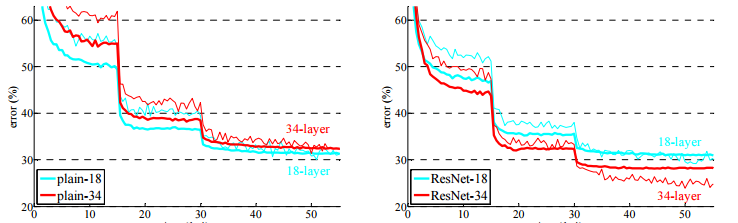
\includegraphics[width=400pt]{Figures/plain_residual_charts.PNG}
\caption{Графики на резултатите при 16 и 34 слоя за стандартни и остатъчни мрежи \cite{He2015} }
\label{fig:plain_residual_charts}
\end{figure}

\begin{figure}[H]
\centering
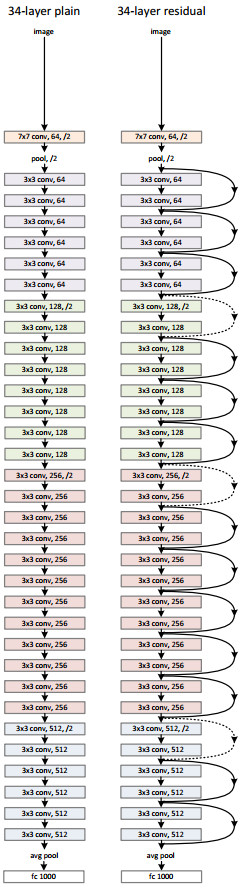
\includegraphics[height=620pt]{Figures/plain_residual.PNG}
\caption{Сравнение на архитектурата на стандартна и остатъчна мрежа \cite{He2015} }
\label{fig:plain_residual}
\end{figure}

Първоначално изображенията се намаляват до размери [256, 480], след което се взима произволен участък с размери [224, 224]. За класификационната задача тестовете са извършени върху 1000 класа с 1 280 000 тренировъчни изображения и 50 000 тестови.

Изпробвани са остатъчни невронни мрежи с 16, 34, 50, 101 и 152 слоя. Има и 2 вида мерки за точност: при първия (top 1) се връща само 1 клас и точността е процентът изображения, за които правилният клас е избран. При втория (top 5) един опит се счита за успешен ако търсеният клас е един от първите 5 върнати класа от невронната мрежа. Най-добрите постигнати резултати са с мрежа със 152 слоя (19.38\% и 4.49\% грешка съответно за top 1 и top 5) \ref{tab:table_results_architectures}.

\begin{longtable}{ | c | c | c | }
\hline
\textbf{Модел} & \textbf{top 1 грешка} & \textbf{top 5 грешка} \\ \hline \hline
ResNet-34 B & 21.84 & 5.71 \\ \hline
ResNet-34 C & 21.53 & 5.60 \\ \hline
ResNet-50   & 20.74 & 5.25 \\ \hline
ResNet-101  & 19.87 & 4.60 \\ \hline
ResNet-152  & \textbf{19.38} & \textbf{4.49} \\ \hline
\caption{Резултати при различните архитектури на невронни мрежи \cite{He2015} }
\label{tab:table_results_architectures}
\end{longtable}
